\section{Интерпретация результатов}

	Согласно статье C. Мотта \cite{black_hole} рентгеновские пульсары, конкретно аккрецирующие черные дыры --- транзиетные системы, т.е. они меняются от длинных <<спокойных>> периодов до коротких вспышек. Такие процессы длятся порядка дней, недель или месяцев, поэтому за ними удобно наблюдать, ведь необходимость вести длинные наблюдения почти отсутствует. Такие систематические изменения (вспышка, например) в спектре черной дыры являются следствием  изменений в аккреционном диске. Само состояние можно описать с помощью шаблонов отслеживаемых на диаграмме твердости-интенсивности. Под интенсивностью подразумевается скорость счета фотонов, а под твердостью подразумевается эквивалент фотометрического индекса цвета; он рассчитывается как $HR = \frac{H + S}{H - S}$, где где H и S - скорости счета данного телескопа в заданных жестких (H) и мягких (S) полосах. На рис. \ref{img:sz} показана типичная форма кривой диаграммы.
	
	\begin{figure}[h!]
		\centering
		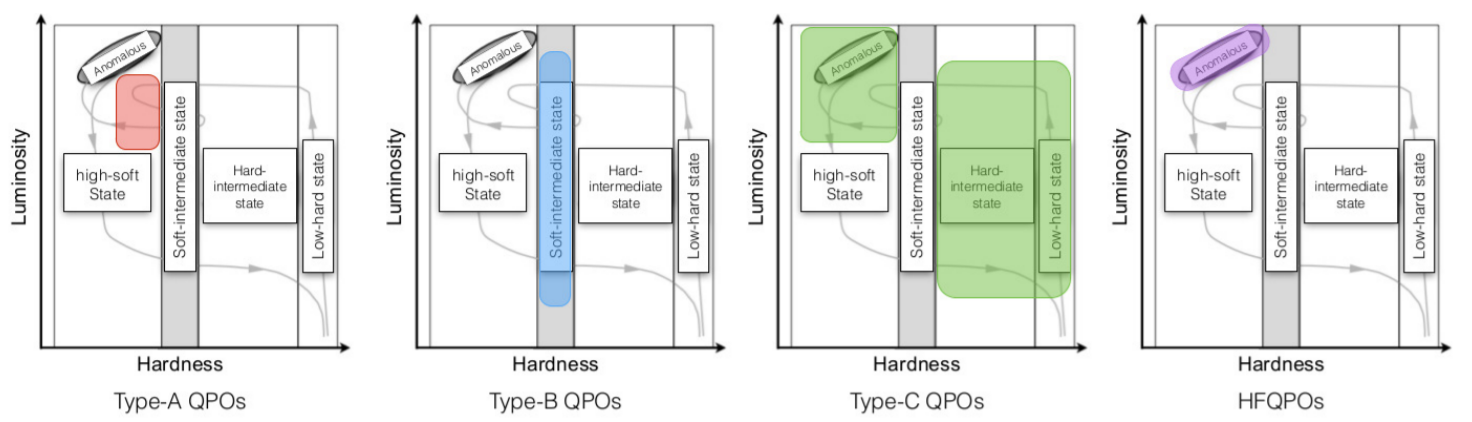
\includegraphics[width = \linewidth]{pictures/HID.png}
		\caption{Типичная диаграмма твердости-интенсивности для черной дыры. Кривая поделена на пять спектральных состояний, также отмечено в каком состоянии проявляются какие QPO}
		\label{img:sz}
	\end{figure}
	
	Пять спектральных состояний различаются по способу излучения, а именно:
	
	\begin{enumerate}
		\item 	Low Hard. В этом состоянии основной источник излучения --- комптоновское эмиссия
		\item High Soft. Здесь источник излучения --- нагретый аккреционный диск
		\item Hard Intermediate и Soft Intermediate. В этих двух состояниях спектр состоит как из жесткого компонента (джет, например), так и теплового излучения диска.
		\item Аномальное. Отличие от Hard Intermediate и Soft Intermediate состоит в том, что светимость объекта значительно выше, чем при последних. 
	\end{enumerate}
	
	\newpage
	
	Квазипериодические осцилляции разделяют на несколько типов: A, B, C и высокочастотные осцилляции. Каждый из типов осцилляций характерен для своего спектрального состояния черной дыры.
	
	Поскольку мы знаем, что частота квазипериодических колебаний MAXI J1820+070 лежит в пределах от $0{,}03$ до $0{,}1$ Гц. Типичные частоты для квазипериодических колебаний типа C лежат примерно в таких пределах, что означает, что черная дыра находится в состоянии Hard Intermediate и сами колебания относятся к типу C. На рис. \ref{img:approx} представлено, как менялась частота колебаний у объекта.
	
	\begin{figure}[h!]
		\centering
		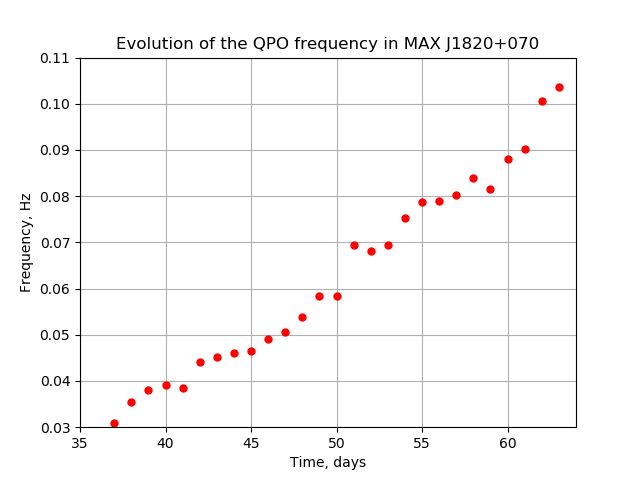
\includegraphics[width = \linewidth]{result}
		\caption{График зависимости частоты квазипериодических колебаний от дня наблюдения}
		\label{img:approx}
	\end{figure}

	Скрипт и остальные графики аппроксимации расположены в Github: 
	
	\url{https://github.com/Grindegreen/report}